\chapter[语言建模基础]{大语言模型的语言建模基础}\label{chap:llm}

\begin{learningbox}
本章将介绍如何在机器学习模型中处理自然语言。具体而言，学完本章后，你将能够：
\begin{itemize}[leftmargin=*, nosep]
    \item 描述{\em 语言建模（language modeling）}的核心概念，包括词元化（tokenization）与早期的词表示方法，并解释每种方法旨在解决什么问题。
    \item 区分构建语言模型所采用的学习方式——{\em 监督学习（supervised learning）、自回归学习（autoregressive learning）与强化学习（reinforcement learning，RL）}——并说明各自对最终模型有何贡献。
    \item 解释{\em 嵌入（embedding）}如何用向量表示词义，并预测语义相关的词在向量空间中的相对位置。
    \item 解释{\em 注意力机制（attention mechanism）}如何在词元之间建立灵活且依赖上下文的连接，并针对给定输入，梳理查询（query）、键（key）与值（value）如何相互作用。
    \item 描述如何以注意力为基础构建 {\em Transformer 架构}，并指出其主要组成部分。
    \item 比较{\em 编码器（encoder）}模型（用于分类）与{\em 解码器（decoder）}模型（用于生成），并针对给定的自然语言处理任务选择合适的模型。
\end{itemize}
\end{learningbox}

\section{自然语言处理}\label{sec:processinglanguage}
语言是人类交流的主要媒介，其形式涵盖纸质书籍、数字媒体与口头话语。长期以来，语言一直是多学科研究的一个重点。在人工智能与计算机科学中，语言尤为重要：我们用它表达复杂思想，用编程语言表述算法，也用它促进软件与用户之间的交互。

正如 \citet{jm3} 在这一领域的重要教材中所指出的，数十年来，人工智能的一项核心目标，就是使机器能够理解人类产生的语言。这方面的研究汇集于自然语言处理（natural language processing，NLP）及其相应的计算语言学（computational linguistics）领域。\footnote{这两个领域最初相距较远，近年来则逐渐靠近；一个从语言学一侧出发，另一个从计算一侧出发。}本章将概述用计算手段把握{\em 自然}（人类）语言的复杂性，并梳理多年来为实现这种理解而发展起来的各项基础技术。

这一领域的早期目标之一，是实现实用机器翻译的梦想。自 20 世纪 50 年代起步以来 \citep{hutchins-1999-retrospect}，人类语言处理技术已经有了长足发展。持续积累的研究进展，使其对各行各业产生了深远影响。反过来，工业界的广泛采用，又成为应用导向发展的重要驱动力。在自然语言处理中，基础理论研究与现实中的实际用途相辅相成，应用范围也因此超出了机器翻译。

\begin{figure}[tb]
    \centering
    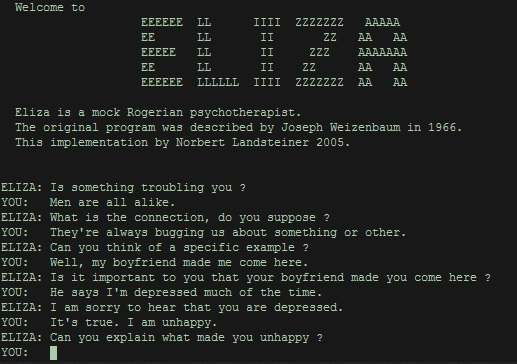
\includegraphics[width=0.7\linewidth]{part1/visuals/ELIZA_conversation.jpg}
    \caption{与 ELIZA 进行的一段典型对话}
    \label{fig:eliza}
\end{figure}

近来，语言技术对社会的影响呈爆发式增长。我们每天都会与 ChatGPT、Claude 等聊天机器人交互，可以使用多种语言；增强型搜索引擎也已融入许多流行产品。不过，这些发展建立在大量早期成果之上。一个著名的早期例子是 ELIZA：Joseph Weizenbaum 于 1966 年开发的心理治疗师聊天机器人 \citep{10.1145/365153.365168}。ELIZA 是一个相当简单的聊天机器人，依据简单规则替换词语（见图~\ref{fig:eliza}）。即使是这样的 ELIZA，也已经被赋予了类似人类的特质。从早期依靠规则处理文本、依据特定分隔符（例如空白字符）识别单词的系统出发，我们如今已经走过了很长的道路。

\subsection{语言理解与语言生成}
在考察计算机如何处理语言之前，我们先看看人类如何理解语言。

一个关键观察是，交流是一个序列过程，语言也相应地形成了序列结构。人们一次说出一个词，也一次接收一个词。人类处理语言与机器处理语言，在这一点上是相通的：语言是字符序列（阅读时）、音节序列（说话时），或完整单词的序列（在早期语言计算模型中）。

下面进一步考察为处理自然语言序列而开发的技术。这些技术可以分为自然语言{\em 理解}与自然语言{\em 生成}两类，我们将分别作简要介绍。

\begin{figure}
    \centering
    % 原图为 part1/visuals/nlp_pipeline.pdf 第 1 页中的 CoreNLP 系统示意图。
% 各分析器与标注对象双向连接；执行流单独向下，不新增分析器间的边。
\resizebox{.95\linewidth}{!}{%
\begin{tikzpicture}[
    font=\small,
    analyser/.style={draw,rounded corners=2pt,fill=blue!5,minimum width=4.4cm,minimum height=.54cm,align=center},
    object/.style={draw,rounded corners=5pt,fill=green!6,minimum width=2.2cm,minimum height=7.5cm,align=center},
    doc/.style={draw,fill=yellow!8,minimum width=1.55cm,minimum height=1cm,align=center},
    flow/.style={-{Stealth[length=2mm]},line width=.7pt}
]
\node[object] (obj) at (6.1,0) {标注对象};
\foreach \name/\yy/\zh/\code in {
    tok/3.35/词元化/tokenize,
    sent/2.4/分句/ssplit,
    pos/1.45/词性标注/pos,
    lemma/.5/形态分析/lemma,
    ner/-.45/命名实体识别/ner,
    parse/-1.4/句法分析/parse,
    coref/-2.35/共指消解/dcoref,
    other/-3.3/其他标注器/{gender, sentiment}}
{
    \node[analyser] (\name) at (1.8,\yy) {\zh};
    \node[font=\ttfamily\scriptsize,anchor=north,inner sep=1pt] at (1.8,\yy-.28) {(\code)};
    \draw[<->,>=Stealth,line width=.6pt] (\name.east) -- (\name.east -| obj.west);
}
\node[doc] (raw) at (9.1,1) {原始文本};
\node[doc] (annotated) at (9.1,-1.5) {已标注文本};
\draw[flow] (raw.west) -- (raw.west -| obj.east);
\draw[flow] (annotated.west -| obj.east) -- (annotated.west);
\draw[flow] (-.9,3.65) -- node[rotate=90,above,inner sep=4pt] {执行流} (-.9,-3.8);
\end{tikzpicture}%
}

    \caption{标准自然语言处理流程，依据 \citet{manning-etal-2014-stanford} 的示意图重绘}
    \label{fig:nlp-pipeline}
\end{figure}

\paragraph{自然语言理解}
自然语言理解（natural language understanding，NLU）着重研究如何捕捉意义与意图。其方法与技术将非结构化的人类语言要素映射为结构化格式，使计算机能够解释这些要素并据此行动。这类技术可以包含受语言学分析启发的多层处理（见图~\ref{fig:nlp-pipeline}），具体如下：
\begin{itemize}
    \item 词元化：确定有意义的语言要素（例如单词）之间的边界，以便进一步处理。
    \item 句法分析（syntactic parsing）：确定语法结构，例如主语、动词与宾语。
    \item 命名实体识别（named entity recognition，NER）：识别人名、日期、地点等关键实体，并对其分类。
    \item 情感分析（sentiment analysis）：检测文本的情感基调。
    \item 共指消解（co-reference resolution）：确定指称表达指向哪个人或事物，例如“{\em 那台计算机}和我说话了”。
    \item 篇章分析（discourse analysis）：理解先前的句子如何影响当前句子的意义。
\end{itemize}
自然语言理解的一项主要挑战，是处理歧义 \citep{DBLP:conf/aaai/Roth98, liu-etal-2023-afraid}。人类语言充满歧义。例如，多义现象意味着一个词有多个含义，如 {\em bank}；还有一些依赖上下文的细微差别，需要借助世界知识才能正确理解。除此之外还有许多挑战；自然产生的人类语言，与人类本身一样丰富而复杂。

\paragraph{自然语言生成}
自然语言生成（natural language generation，NLG）着重研究如何产生可读、自然的人类语言，任务范围既包括自由形式的语言生成，也包括将结构化数据或模型表示转化为逼真的话语。

自然语言生成中的一项重要任务是\emph{语言建模（language modeling，LM）}。在语言建模中，任务是根据先前的上下文预测序列中的下一个元素。从数学上说，这需要为词语序列赋予一个概率分布。传统方法通常使用简单的计数模型来求取这一分布，并且往往采用进一步的简化假设，根据前面固定窗口内的词语预测下一个词。

现代方法使用复杂的神经网络技术，能够依据较长的上下文生成流畅的句子，这些句子在人类观察者看来往往是有意义的。\footnote{从 ELIZA 的例子可以看到，单是做到这一点，并不总是很困难。}需要注意，有效的语言生成不仅要求语法正确，还要求连贯性（逻辑上的流畅）与衔接性（语言层面的联系）。当前的自然语言生成系统使用采样、集成及许多其他机制，在所生成文本的创造性与可预测性之间取得平衡，使输出显得自然，而不是机械生硬 \citep{li-jurafsky-2017-neural, 10.1145/3554727, gatt2018survey}。自然语言生成技术通常分为两种方法：
\begin{itemize}
    \item 抽取式生成（extractive generation）：选择并重新排列已有的文本片段，常见于早期的摘要工具。
    \item 抽象式生成（abstractive generation）：从零开始生成全新的句子，ChatGPT 等现代模型即采用这种方式。
\end{itemize}
大多数大语言模型采用抽象式方法。

接下来，我们讨论语言建模早期的一些基础方法。我们先介绍语言的复杂性，再讨论分布表示原理、词元化方法，以及早期的语言建模表示。

\subsection{自然语言的复杂性}
自然语言之所以难以让机器解释，原因有很多。语言中的细微差别能够传递意义，也能够扭曲意义。要捕捉语言的全部细节，仅理解其结构还不够。此外，话语所处的上下文也会影响交流。理解需要超越词语本身，领会交流中蕴含的意图、隐含意义与微妙之处 \citep{wittgenstein1953philosophical, Grice_1975, krause-vossen-2024-gricean-maxims}。下面介绍语言学研究中的几个主题；每个主题都从不同角度，考察语言能够表达什么。

\paragraph{句法} 句法（syntax）规则支配句子的结构。在语言学中，句法指的是制约某种语言句子结构的一套规则、原则与过程。语言句法研究其背后的逻辑：说话者如何把词组合为形式合规且具有意义的序列。例如，在英语中，最常见的语序是主语—动词—宾语；在 {\em cat bites dog} 中，动词 {\em bites} 位于主语 {\em cat} 之后，表明这句话说的是猫在咬，而不是狗在咬。

\paragraph{形态学} 形态学（morphology）研究词语如何随其语法功能而改变形式。词形变化与句法有关，形态规则及其例外则取决于具体语言或语系。在前面的例句中，动词 {\em to bite} 变成了 {\em bites}，其中的 {\em -s} 表示一般现在时：事情正在发生，施事者是单数，而不是远古时代的一群猫。

\paragraph{语义学} 在语言学中，词汇语义学（lexical semantics）研究词语的意义。在自然语言中，词义源于词与其他词之间的关系。例如，意义几乎相同的词构成{\em 同义词}，如 car 与 automobile，或 vanish 与 disappear；意义相反的词构成{\em 反义词}，如 hot 与 cold，或 buy 与 sell。此外还存在许多其他关系。

在自然语言处理中，计算语义学（computational semantics）研究如何在计算机中高效表示这些意义。把一个句子存入计算机内存时，一种基本方法是建立一个包含某种语言全部词语的向量，再用指向该向量的索引序列表示句子。不过，这种编码只记录词语的出现，没有记录词与词之间的关系；词语的语义已经不在这种朴素表示之中。

词语的意义来自它与其他词之间的关系，因此我们需要高效编码这些关系的方法。正如本章后面将看到的，多年来，人们已经提出了不同方案，包括 Transformer 架构与注意力机制。

\paragraph{语用学} 除了词语的字面意义，人们还关心说话者的意图与话语所处的上下文。语言在特定社会情境中的使用方式，决定了它的作用（{\em 意义即使用} \citep{baker2008wittgenstein}）。人类为了让交流有效，会自然而然地遵循一些隐含的日常规则；研究这些规则的学科称为{\em 语用学（pragmatics）}。

Grice 合作准则（Gricean Maxims）是一组奠基性的原则 \citep{Grice_1975}，即人类用来推知意义、无需明说的合作原则。例如，数量准则要求人们提供的信息恰好满足会话需要。这些准则塑造了我们的交流，帮助语言变得可理解且具有合作性。机器要理解反讽、言外之意，或“thingy”（那个东西）这样的占位表达，仅遵循静态词典还不够，还需要了解这些规则。

\paragraph{篇章} 语言很少以孤立句子的形式出现，而是组织成段落、会话或完整文档等更大的单位。篇章（discourse）研究关注句子如何相互连接，形成既衔接又连贯的整体。机器要真正解释一篇文本，就必须能够在多个句子中追踪实体，这项任务称为共指消解，例如确定代词 {\em it} 指的是前一句中的猫、狗，还是那次咬伤。对于文档摘要、机器翻译与长对话维持等复杂自然语言处理任务而言，理解篇章至关重要。

除上述主题外，还有语音学（研究语言中的声音，以及这些声音在人类交流中承载的额外意义）、社会语言学（研究语言如何随阶层、地域等社会因素而变化）、词典学（编纂词典的学问）等许多研究领域。

从这番概览可以看出，自然语言生成与理解都是庞大而富有挑战的领域。还应认识到，语言不是静止不变的。语言会随时间、地理位置、文化以及交流媒介而变化 :-)。
这种变异使语言技术的创造成为一项艰巨且永无止境的探索。

在介绍近期那些至少能部分应对上述挑战的技术之前，我们先讨论推动自然语言处理迈向现代方法的基本假设。

自然语言丰富而复杂，因此很难在计算机中表示。本节余下部分将讨论分布表示原理：词语的语义由其周围的上下文所驱动。随后介绍词元化方法，即将句子切分为词语的方法。最后，我们讨论如何利用词元向量，得到能够编码意义的表示。

\subsection{分布表示}
如果不手工编码所有复杂的语义关系与语法结构，怎样教会机器理解它们？答案在于分布假设（distributional hypothesis），这是现代自然语言处理的一个基础概念。其核心思想在 20 世纪 50 年代末得到了如下表述：
\begin{center}
    \emph{观其常伴之词，即可知其词义。（Firth，1957）}
\end{center}
这意味着，可以根据某个词通常出现时周围的词语，即上下文，推知它的意义。出现在相似上下文中的词语，很可能具有相似意义。例如，如果 {\em coffee} 与 {\em tea} 都经常出现在 {\em drink}、{\em sip} 或 {\em brew} 这样的动词附近，那么，即使没有明确定义或其他由人提供的信息，机器也可能判断这两个词之间存在语义关系。

为了使分布假设能够用于计算，我们借助线性代数，采用一种称为\emph{向量语义（vector semantics）}的框架，把词语表示为高维连续空间中的点。意义相似的词会映射到这个空间中彼此接近的点，我们便可以用余弦相似度等几何距离度量来衡量语义相似性（见图~\ref{fig:word-embeddings}~及第~\ref{sec:cosine}~节）。此外，还可以通过向量运算改变词语的意义。
早期实现依靠稀疏共现矩阵构造语义向量，在每个词的上下文中计数，这与第~\ref{sec:early}~节描述的其他方法很相近。现代方法更倾向于使用稠密的低维向量，通常称为\emph{词嵌入（word embedding）}。这些表示通常通过训练神经网络模型来学习：根据相邻词预测某个词，或反过来根据某个词预测相邻词。\emph{word2vec} 架构使这一突破广为人知 \citep{mikolov2013efficient}。

虽然学习词语的向量表示能够有效捕捉意义，但如果为一种语言中的每个不同单词都保留一个独立向量，词表就会庞大到不切实际。

此外，严格以完整词语为单位的方法，很难处理罕见词或从未见过的词，因为模型事先没有这些词的向量。因此，在模型能够为语言单位赋予向量之前，我们首先必须确定，基本单位究竟是什么。为了消除这些低效之处并处理词表外输入，现代方法系统地将原始文本拆解成更便于处理的片段。这个过程称为词元化，下面就来介绍。

\begin{figure}
    \centering
    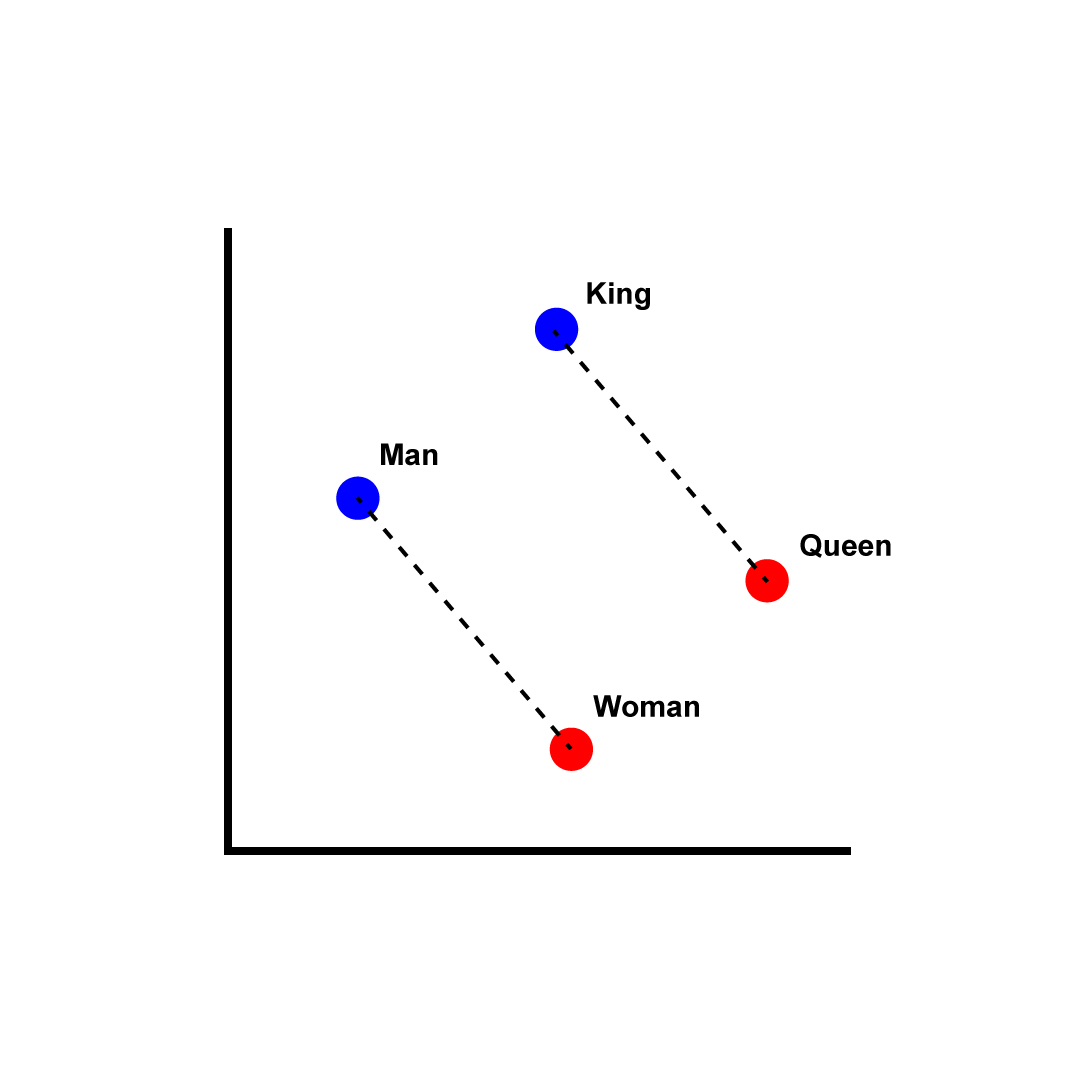
\includegraphics[width=0.52\linewidth,trim=200bp 200bp 170bp 200bp,clip]{part1/visuals/Word_vector_illustration.jpg}
    \caption{使用 word2vec 词嵌入进行向量运算的示意图 \citep{singerep2022wordvector}。}
    \label{fig:word-embeddings}
\end{figure}

\subsection{词元化}
\label{sec:tokenization}
在计算机能够为语言赋予意义之前，必须先找到吸收语言的方式。假设我们已经取得了原始文本，无论它们来自网页抓取还是语音转写，眼前的挑战都是：如何把连续的字符串切分为有意义的单位，或者说，如何把句子切分为词语。这一过程称为\emph{词元化}。不过，稳健的词元化策略所做的，远不止按空格分词；它还必须应对不同语言和方言的细微差别，分析复杂的标点用法，甚至考虑表情符号等现代新增元素，并将它们纳入大小固定的词表。

切分是许多自然语言处理流程中的关键步骤。划分文本看似简单，标点中的歧义却会使过程复杂化，例如缩写究竟应写作 N.L.P. 还是 NLP？简单的基于规则的切分器，面对自然语言结构中的不规则现象时，经常会失效。因此，人们提出了构造这些单位的不同方法，见例~\ref{ex:tokenization}。

\begin{example}[词元化策略]\label{ex:tokenization}
考虑下面这句话：\\ ``Leiden is beautiful in summer.''

\vspace{0.3cm}
\noindent\textbf{词级词元化} \\
这种方法通常根据空格与标点切分文本。\\
\vspace{0.1cm}
\noindent\texttt{["Leiden", "is", "beautiful", "in", "summer", "."]}

\vspace{0.4cm}
\noindent\textbf{字符级词元化} \\
这种方法把文本拆分为单个字符。\\
\vspace{0.1cm}
\noindent\texttt{["L", "e", "i", "d", "e", "n", " ", "i", "s", " ", "b", "e", "a", "u", "t", "i", "f", "u", "l", " ", "i", "n", " ", "s", "u", "m", "m", "e", "r", "."]}

\vspace{0.4cm}
\noindent\textbf{子词词元化（例如 WordPiece）} \\
这种方法把常见词保留为完整词元，同时将复杂词或罕见词拆成基本子词。\\
\vspace{0.1cm}
\noindent\texttt{["Lei", "\#\#den", "is", "beautiful", "in", "summer",}\\
\noindent\texttt{"."]}
\end{example}

\paragraph{词级词元化}
这种方法将每个以空格分隔的字符串视为一个独立词元。它虽然保留了句法结构，却会造成大得不切实际的词表，而且存在词表外（out-of-vocabulary，OOV）问题：模型无法处理训练时未曾见过的词。

大词表之所以成问题，与\emph{独热编码（one-hot encoding）}的机制有关。如果词表 $V$ 中的每个词 $w$ 都表示为向量 $\mathbf{x} \in \{0, 1\}^{|V|}$，其中只有对应于 $w$ 的位置取值为 1，那么维数 $|V|$ 就会随词表大小线性增长。这些独热向量随后会成为神经网络的输入；对于没有包含词表中全部词语的文本，我们最终得到的表示既稀疏、计算效率又低，还无法捕捉词与词之间的语义关系。

\paragraph{字符级词元化}
纯字符级建模似乎能够直接解决词表不断增大的问题，多年来也已有许多探索 \citep{mielke2021wordscharactersbriefhistory}。这种方法把文本切分为单个字符，使词表大小限制在字母表的规模，几乎消除了词表外问题。不过，它显著增加了序列长度，带来相当大的计算负担。此外，孤立字符本身缺乏固有的语义，模型必须先学习词的形态，才能把握更广泛的语言规律，因此训练时间也会增加。

\paragraph{子词词元化} 因此，当前大语言模型采用的标准方法，是在前两种方法之间取得平衡：将常见词保留为完整词元，把罕见词拆解为更小且有意义的组成部分。代表性实现包括：

\begin{itemize}
    \item 字节对编码（byte pair encoding，BPE）：一种迭代算法，从单个字符出发，不断把频率最高的相邻二元组并为一个词元，直到达到目标词表大小 \citep{sennrich-etal-2016-neural}，例如 \textit{highest} $\rightarrow$ [\textit{high}, \textit{est}]。BPE 最初是作为数据压缩算法提出的 \citep{gage1994new}。
    \item WordPiece：一种与 BPE 相似的迭代算法，但它根据似然准则合并二元组，而不是依据原始频数，目标是最大化训练数据的概率 \citep{wu2016googlesneuralmachinetranslation}。
\end{itemize}

\subsection{早期的语言表示方法}
\label{sec:early}
词元化之后，下一个问题是：如何把语言单位，也就是词元，组合成连贯且承载意义的句子？我们先注意到，人类语言中这些单位的顺序受严格的句法与语义规则支配。如果计算方法能够准确地产生有意义的文本序列，那么我们或许可以说，它们具有同样的句法与语义理解，至少也能够复现这样的理解。

如何构建数学表示来实现这一目标？其中的一项核心任务就是\emph{语言建模}。从数学上说，语言模型是一个函数，用来计算词语序列在特定上下文中共同出现的联合概率。通过计算这个概率，模型能够区分逻辑合理、表达流畅的句子与随机词元序列。例如，在英语中，\textit{the cat sat} 比 \textit{sat cat the} 的概率大得多，因为前者遵循既有的句法规则。

书面语言具有序列性，因此，估计一个句子的联合概率，本质上是序列估计问题。语言建模的总体目标，是根据句子 $S$ 所包含的词语序列 $w_1, \dots, w_k$，量化它在某种语言中出现的统计可能性：

\begin{equation}
    \label{eq:language-sequence}
    P(S) = P(w_1, \dots, w_k)
\end{equation}

对于任意长度的句子，直接计算这一精确联合概率在计算上不可行，因为在给定词表中，可能的词语组合数量呈指数增长。为了化解这种复杂性，我们通常利用概率的链式法则分解联合概率。再对条件独立性作出特定的数学假设，就能够使计算在实际应用中保持可处理性 \citep{jm3}：

\begin{equation}
\label{eq:bigram}
    P(w_1, \dots, w_k) = P(w_1) \prod_{i=2}^{k} P(w_i \mid w_1, \dots, w_{i-1})
\end{equation}

通过最大化这一联合概率，概率模型学会偏好语法正确、逻辑合理的序列。学到的概率分布，实际上是在反向重建人类语言中复杂且未明确写出的规则 \citep{manning1999foundations}。为了从切分后的文本语料中估计这些概率，早期方法采用最大似然估计（maximum likelihood estimation，MLE）。最简单的方法根据词在语料中的相对频率计算其边际概率：

\begin{equation}
\label{eq:mle-word-prob}
    P(w) = \frac{\text{count}(w \text{ in corpus})}{\text{total number of words}}
\end{equation}

为了使这些条件概率的计算易于处理，研究者采用 \emph{$n$ 元模型（n-gram model）}。$n$ 元组是给定文本样本中连续出现的 $n$ 个元素所构成的序列。给定某个词之前的完整历史来计算其概率，很快就会变得难以处理；$n$ 元模型则采用\emph{马尔可夫假设（Markov assumption）}，认为下一个词的概率仅取决于前面的 $n-1$ 个词，从而截短上下文。例如，二元模型（$n=2$）只看紧邻的前一个词，以此近似完整历史。条件概率的计算方式，是把两个词共同出现的频数，除以前一个词单独出现的频数：

\begin{equation}
    P(w_i \mid w_1, \dots, w_{i-1}) \approx P(w_i \mid w_{i-1}) = \frac{\text{count}(w_{i-1}, w_i)}{\text{count}(w_{i-1})}
\end{equation}

类似地，三元模型（$n=3$）以前面的两个词为条件。这种简化显著降低了计算负担，使直接从语料中估计概率成为可行之举。

选择合适的 $n$，需要作出一项重要权衡。较大的 $n$ 能够捕捉更丰富的上下文信息与更深的句法依赖，使模型生成更自然的语言。不过，随着 $n$ 增大，稀疏性问题会以指数速度恶化：高度特定的词语序列在训练数据中出现得少得多，模型遇到零概率的情况也会越来越多。反之，较小的 $n$ 可以得到稳健且频繁的计数，却严重限制了模型对较广泛语义及句内长距离依赖的理解。

在标准语言模型的计算中，一个未见过的 $n$ 元组会得到零概率，进而通过乘法使整个句子的联合概率归零。为了缓解这种反直觉的现象，通常会对计数进行平滑。一种常用技术是\emph{拉普拉斯平滑（Laplace smoothing）}，也称加一平滑，即给每个可能的词表项添加一个虚拟计数 $1$。为维持有效的概率分布，分母也要加上词表大小 $|V|$：

\begin{equation}
\label{eq:mle-word-prob-laplace}
    P_{\text{Laplace}}(w) = \frac{\text{count}(w \text{ in corpus}) + 1}{\text{total number of words} + |V|}
\end{equation}

这些基于概率与计数的方法，最终得到的是语言的数值表示。好的表示应当编码我们直觉上能够把握的词语属性：词义、语法功能，以及它与其他词之间的关系。在早期自然语言处理中，人们把这些相对频率与共现计数组织成向量，根据词在文本中的分布表示词语。

基于计数的表示虽然可以计算，却会产生高维稀疏向量，导致计算低效，并且在未见数据上的泛化能力较差。因此，现代自然语言处理转而使用神经网络，学习称为\textit{嵌入}的稠密低维向量表示。这些模型不依靠显式计数，而是在根据周围上下文预测词语的过程中，附带学到连续表示，以更高效的形式捕捉更深的语义关系。第~\ref{sec:modernNLP}~节将讨论这些现代方法。在此之前，我们先稍作停顿，回顾三种重要的机器学习方法。

\section{自然语言处理中的机器学习方法}
\label{sec:machinelearning}
\chaptermark{自然语言处理中的机器学习方法}
介绍了语言表示的基础知识后，我们现在转向学习算法；正是这些算法，使我们能够构建支撑现代人工智能系统的大型模型。大语言模型的训练方法来自更广泛的机器学习领域。机器学习的研究范围十分广阔，而理解大语言模型，需要熟悉三个核心范式，以及它们在语言建模中的用法：\emph{监督学习}、\emph{自回归学习}与\emph{强化学习}。我们将简要介绍这些必要方法，更深入的内容请参阅相关经典著作。

\subsection{监督学习}
监督学习是机器学习的基础。它之所以这样命名，是因为它依赖一组必须预先给出的标签，由这些标签\textit{监督}训练过程。这种方法使用由样例与标签成对组成的数据集 $D = \{(x_i, y_i)\}$，训练预测模型 $f_\theta$ 的参数 $\theta$。模型可以为每个输入 $x$ 计算估计值 $\hat{y}$，数学上记作 $f_\theta(x) \rightarrow \hat{y}$。使用模型计算这一估计值，也称为{\em 推理（inference）}或{\em 前向传播（forward pass）}。

前向传播之后，我们可以使用损失函数 $\mathcal{L}$，计算估计值 $\hat{y}$ 与真实标签 $y$ 之间的某种差异。常见的损失函数包括统计回归中的平方差之和 $\mathcal{L} = \sum_i(\hat{y_i} - y_i)^2$，以及分类中的交叉熵损失 $\mathcal{L} = -\sum_cy_c\log(\hat{y_c})$。

监督训练算法的目标，是通过调整参数，使样例对数据集上的损失总和最小。这一步在{\em 反向传播（backward pass）}中完成：根据损失函数计算误差信号，调整模型 $f$ 的参数 $\theta$，使下一次前向传播取得更低的损失，也就是对误差进行反向传播。最小化数据集样例上损失函数的过程，称为\emph{训练（training）}。在全部训练数据上完成一轮前向与反向传播，称为一个\textit{训练轮次（epoch）}；出于效率考虑，每个训练轮次又可以划分为多个训练\textit{批次（batch）}。

训练完成后，为了检验模型 $f_\theta$ 是否工作良好，也就是能否泛化到未见过的样例，需要在未参与训练的新样例上进行\textit{测试}。

如果模型在训练集上的准确率很高，我们就说模型训练得很好，即训练收敛。如果在测试集上的准确率也很高，就说明模型泛化良好，达到了训练目标。通俗地说，如果模型在训练集上准确率很高，在测试集上却很低，我们就说模型对训练集过拟合（overfitting）。这通常意味着模型训练过久，或参数过多，以至于除了拟合训练集中的信号，还拟合了噪声。如果模型在训练集与测试集上的准确率都很低，则称为欠拟合（underfitting）。这很可能是训练时间太短，或模型过于简单、可训练参数太少，不足以刻画数据中的复杂性。

一般而言，变量较少的低维问题，例如简单回归，使用较小的模型、较少的参数与训练数据，就能取得良好表现。变量较多的高维问题，例如图像分类，则需要具有数百万参数的大模型（通常是深度神经网络）和大型训练数据集，才能表现良好。事实上，图像分类取得突破性性能 \citep{krizhevsky2012imagenet}，是在包含数百万张人工标注图像的大型数据集 Imagenet 建成之后 \citep{deng2009imagenet}。

监督学习是机器学习的基础，已有许多优秀教材介绍这一主题 \citep{bishop2023deep,goodfellow2016deep}。它也是大语言模型训练的核心技术之一，例如用于监督微调；下一章将介绍这一点。

\subsection{自回归学习}
大语言模型采用自回归方式训练。这种训练方法没有成对的标注样例数据集，却有大量可用的文本等数据。自回归学习是一种不使用显式标签的自监督学习（self-supervised learning），利用数据内在的序列性来预测下一个词元。

在语言模型的自回归预训练中，算法在数据集上进行预测，将每个词元 $y=x_t$ 作为其前面样例词元 $\mathbf{x}=x_{t-1}$ 的标签。自回归学习是现代自然语言处理的核心任务，已用于当代模型的训练流程 \citep{radford2018improving}，也已写入自然语言处理教材 \citep{jm3}。第~\ref{sec:modernNLP}~节与第~\ref{chap:pipeline}~章将进一步介绍这些方法。

\subsection{强化学习}
\label{sec:sdp}\label{sec:rl}
监督学习与自回归学习都需要训练数据集，在预先存在的数据上进行{\em 离线（offline）}训练。不过，有时我们没有现成数据集，却可以使用一个函数，判断当前处于好状态还是坏状态。此时，可以采用称为强化学习的{\em 在线（online）}学习方法：智能体执行动作 $a$，使环境从状态 $s$ 转移到下一个状态 $s'$，随后环境返回新状态的奖励 $r(s')$。之所以称为在线，是因为方法在训练的同时即时生成训练数据。智能体可以利用奖励信息，调整由参数 $\theta$ 表征的行为策略函数 $\pi_\theta(s) \rightarrow a$，学习在什么状态下执行什么动作。当所处理的是序贯决策问题时，动作 $a$ 使系统从状态 $s$ 转移到另一状态 $s'$，而奖励取决于过去采取的动作；这就产生了信用分配问题（credit assignment problem）：奖励应当归因于哪些动作？反复执行状态／动作／奖励过程，可以使智能体探索整个状态空间，学习在每个状态下应当采取何种动作的最优策略 $\pi^*(s)$。

\begin{figure}[tb]
  \begin{center}
    \input figures/rl
    \caption{强化学习，依据 \citet{sutton2018reinforcement} 绘制}\label{fig:rl-org}
  \end{center}
\end{figure}

需要注意，强化学习是一种在线方法，因此本质上是循环的。开始时，策略 $\pi$ 只见过少量奖励，仅在少数状态下掌握了该采取何种动作的有用信息。如果它贪心地利用这些信息，一味执行已知的好动作，就只会经过环境中有限的一部分，找到的最优策略也只是局部最优。为了找到更好的最优解，它应当进行探索、尝试随机动作，理想情况下应覆盖整个状态空间。

强化学习是智能体主动根据环境反馈进行学习的一种方式。一个关键认识是，判断输出好不好，即构建奖励函数，通常比从头创造一个完整输出、构建标注数据集，更容易。已经提出的许多强化学习算法，都着眼于良好的探索方法。
强化学习问题在形式上建模为马尔可夫决策过程（Markov decision process，MDP），其组成包括状态表示 $S$、动作函数 $A(s)$、转移函数 $T(s, a) \rightarrow s'$ 与奖励函数 $R(s)$。奖励是环境提供的、表示状态质量的数值，可以为正，也可以为负。智能体的目标是找到策略 $\pi(s)$，在每个状态 $s$ 下选取最优动作 $a*$。
图~\ref{fig:rl-org}~展示了强化学习智能体如何通过与环境交互，在线学习一个为每个状态指定动作的策略。环境能够计算函数 $T$ 与 $R$，也就是回答智能体的两个问题：执行动作后到达了什么新状态，以及这个状态有多好。

当状态空间足够小、能够完整放入计算机内存时，可以采用精确的表格型强化学习方法，例如 Q-learning \citep{watkins1992q}。对于更大的问题，则使用基于深度神经网络的函数近似方法，例如深度 Q 学习（deep Q-learning，DQN）\citep{mnih2015human}，或近端策略优化（proximal policy optimization，PPO）\citep{schulman2017proximal}。在深度强化学习中，策略是一个参数化神经网络，与监督深度学习一样，通过反向传播进行训练。

强化学习是现代推理语言模型的基础。有关强化学习的教材很多，例如 \citet{sutton2018reinforcement} 的奠基性著作，以及更侧重教学的著作 \citep{graesser2019foundations,plaat2020learning,plaat2022deep}。在大语言模型训练中，强化学习用于强化微调与多步推理，第~\ref{chap:reasoning}~章将讨论这些内容。此外，强化学习把机器学习问题表述为智能体尝试学习如何与环境交互的过程，与智能体大语言模型的场景十分契合。在智能体大语言模型中，它既用于通过上下文强化学习优化提示，也用于世界模型，以及对其他智能体相对于环境的行为进行建模；本书后面将进一步介绍。

强化学习是一种流行的机器学习方法，因为在没有可用数据时，我们也能够学习新的环境：这种方法会自行获取数据。考虑是否使用强化学习时，应回答两个问题：(1) 当前问题是不是序贯决策问题？如果是，(2) 状态空间有多大，能够使用精确的表格方法，还是必须采用近似方法？

现在，必要的语言与机器学习原理已经介绍完毕，我们回到语言，进入下一步：语言建模。

\section{语言建模}\label{sec:modernNLP}
介绍了语言表示与机器学习的基础知识后，我们转向构建计算语言建模能力所采用的总体范式。自然语言处理的发展大体经历了三个范式。每个范式都代表一次根本转变：构建何种模型来捕捉语言，以及如何应对人类语言固有的复杂性。我们将看到，随着范式演进，越来越多的机器学习技术被纳入其中，人们借助计算能力的提升处理更多数据，训练越来越大的神经网络来处理语言。这三个范式分别是\textit{符号方法}、\textit{统计方法}与\textit{神经网络方法} \citep{kautz2020third, deng2018deep}。

\paragraph{符号方法} 这些类似 ELIZA 的早期符号方法，通常称为\textit{经典人工智能}或基于规则的系统，依赖由人明确定义的指令。符号模型把语言视为形式系统，尝试通过演绎来分析意义。这些系统在设计上高度透明、可解释，却也十分脆弱：它们很难依靠僵硬的规则，如 \textit{if-then-else}，处理现实语言中的自然变异、惯用表达与歧义。把符号方法扩展到更大的语言任务，需要耗费大量人力，手工列举众多边界情况。事实证明，除了最小的问题领域，这条路几乎都不可行。

\paragraph{统计方法} 为克服僵硬规则集的局限，20 世纪 80 至 90 年代，这一领域经历了向经验方法的转向，开始用统计方法进行概率建模。隐马尔可夫模型与 $n$ 元语言模型等统计方法，不依靠明确的句法规则，而是利用大型文本语料计算词语共现的似然。这种数据驱动的方法能够高效扩展，在处理语言歧义与噪声方面，也远胜此前的符号方法。不过，由于这些模型通常采用马尔可夫假设，其意义表示天然局限于局部词语模式，很难捕捉长距离依赖与更广的上下文。

\paragraph{神经网络方法} 大约在 2010 年之后，最先进的方法转向神经网络与深度学习。神经网络方法不再使用逻辑或离散计数，而是在连续语义空间中，用稠密的低维向量表示语言单位。现代架构，尤其是 Transformer，利用注意力机制，同时对整个序列的全局上下文建模。这种方法取得了令人瞩目的泛化能力、流畅的文本生成能力与跨语言能力。不过，这些优势也伴随着显著代价：神经网络模型很大程度上像黑箱一样运作，牺牲了符号方法所具有的可解释性，同时还需要庞大的数据集与计算资源。

当代自然语言处理训练流程从这三种范式中都汲取了灵感。下一章将介绍一个训练流程的例子；在此之前，我们需要更深入地理解其中的核心组成，因为它们正是智能体大语言模型所依托系统的基本构件。下面各小节将讨论词嵌入、上下文相关嵌入、序列建模、注意力、Transformer、编码器（例如 BERT）与解码器（例如 GPT）等主题。

\subsection{嵌入}\label{sec:cosine}
早期神经嵌入模型通过定义上下文窗口，把对词汇项的语义理解转化为可操作的任务：在目标词左右各取 $n$ 个词，预测缺失的中心词。例如，在句子 \textit{There are two cookies left on the table} 中，如果窗口设为 $n=2$，那么 \textit{cookies} 的上下文词就是 \textit{are}、\textit{two}、\textit{left} 与 \textit{on}。在大型文本语料上系统地滑动这个窗口，就能够统计每个词在其他各词的上下文中出现了多少次。这些计数构成共现矩阵的基础：每行代表一个目标词，每列代表一个上下文词，单元格的值表示列中的词在行中词的上下文里出现的次数。例如，\textit{cherry} 的向量在 pie 这一列可能取较高值，如 442，而在 computer 这一列取较低值，如 2。\textit{strawberry} 的向量则会表现出相似模式，从而反映这两个词的语义相似性。

把词表示为向量，就相当于将它们放入一个高维向量空间，每个维度对应一个上下文词。在这个空间中，意义相似、上下文相近的词，会指向相近的方向。这种几何关系使我们能够用数值衡量语义相似性。最常用的方法是\emph{余弦相似度（cosine similarity）}，即度量两个向量 $\mathbf{a}$ 与 $\mathbf{b}$ 夹角 $\theta$ 的余弦，如式~\ref{eq:cosine}~所示。

\begin{equation}
    \label{eq:cosine}
\text{similarity} = \cos(\theta) = \frac{\mathbf{a} \cdot \mathbf{b}}{\|\mathbf{a}\| \|\mathbf{b}\|} = \frac{\sum_{i=1}^{n} a_i b_i}{\sqrt{\sum_{i=1}^{n} a_i^2} \sqrt{\sum_{i=1}^{n} b_i^2}}
\end{equation}

前面已经指出，基于计数的向量会形成高维空间，维数随词表大小线性增长。由于维数决定下游模型的计算复杂度，我们希望控制维数，改为构造稠密嵌入。为此，可以采用经典的 word2vec 算法 \citep{mikolov2013efficient}。这种方法先随机初始化嵌入矩阵 $W$，再迭代更新，使其符合“相似词出现在相似上下文中”这一直觉。这个总体框架通过两种不同技术实现上述目标：跳字模型与连续词袋模型，见图~\ref{fig:word2vec}。

第一种方法是\emph{跳字模型（skip-gram）}，它预测给定目标词周围可能出现哪些上下文词。模型通过更新矩阵，使正样本，即真实的目标词—上下文词对，具有较高余弦相似度，同时降低负样本，即随机词对，之间的相似度。由于跳字模型把每个目标词—上下文词配对都看作一个独立训练观测，即使是低频词，预测错误也会受到较强惩罚。因此，跳字模型擅长捕捉细致的语义特征，即使对罕见词，也能给出准确表示。

第二种方法是\emph{连续词袋模型（continuous bag-of-words，CBOW）}，其操作方向正好相反：根据组合起来的一组周围上下文词，预测一个目标词。由于在预测目标词之前会对上下文向量取平均，连续词袋模型天然会平滑掉各个上下文词的具体细节。这种分布平滑解释了它不同的性能特点：连续词袋模型的训练速度显著快于跳字模型，也很善于捕捉高频词之间一般性的句法关系，但对罕见词的敏感性会有所损失。

\begin{figure}[tb]
    \centering
    \begin{minipage}{0.45\textwidth}
        % 英文词语是原图的训练词元例子，保留不译。
\resizebox{\linewidth}{!}{%
\begin{tikzpicture}[font=\small,word/.style={circle,draw,fill=blue!25,minimum size=.65cm,inner sep=0pt},flow/.style={-{Stealth[length=2mm]},line width=.7pt}]
\node[word,fill=cyan!55] (focus) at (2,0) {};
\node[below=2mm of focus] {loves};
\foreach \id/\xx/\term in {a/0/the,b/1/man,c/3/his,d/4/son}{
  \node[word] (\id) at (\xx,1.3) {};
  \node[above=2mm of \id] {\term};
  \draw[flow] (focus) -- (\id);
}
\end{tikzpicture}%
}

    \end{minipage}
    \hfill
    \begin{minipage}{0.45\textwidth}
        % 英文词语是原图的训练词元例子，保留不译。
\resizebox{\linewidth}{!}{%
\begin{tikzpicture}[font=\small,word/.style={circle,draw,fill=blue!25,minimum size=.65cm,inner sep=0pt},flow/.style={-{Stealth[length=2mm]},line width=.7pt}]
\node[word,fill=cyan!55] (focus) at (2,1.3) {};
\node[above=2mm of focus] {loves};
\foreach \id/\xx/\term in {a/0/the,b/1/man,c/3/his,d/4/son}{
  \node[word] (\id) at (\xx,0) {};
  \node[below=2mm of \id] {\term};
  \draw[flow] (\id) -- (focus);
}
\end{tikzpicture}%
}

    \end{minipage}
    \caption{构建词嵌入的跳字模型（左）与连续词袋模型（右）示意图 \citep{d2l_cbow_2023}。}
    \label{fig:word2vec}
\end{figure}

\subsection{转向上下文相关嵌入}
word2vec 使高质量词嵌入的构建向前迈进了一大步，但它有一个明显缺点：产生的是\textit{静态嵌入（static embedding）}。这意味着，无论一个词如何使用、处于什么上下文，它都映射为同一个向量。这给一词多义带来了根本问题。考虑下面两个不同句子中的 \textit{bank}：
\begin{enumerate}
    \item I need to go to the \textit{bank} to withdraw some money.（我需要去银行取些钱。）
    \item The swimmer sat on the river \textit{bank}.（游泳者坐在河岸上。）
\end{enumerate}
在静态模型中，\textit{bank} 只有一个固定表示，必须在这些相距甚远的意义之间取平均或作出选择，得到的向量既不纯粹属于金融意义，也不纯粹属于地理意义，或者成为两者的奇怪混合。现代架构，例如本章后面将讨论的 BERT 与 GPT，通过产生\textit{上下文相关嵌入（contextualized embedding）}解决这一问题。模型不使用静态查找表，而是处理整个序列，根据周围词元——\textit{money}、\textit{withdraw} 或 \textit{river}、\textit{swimmer}——动态计算 \textit{bank} 的向量，使机器能够表示说话者意指的具体细微含义。

\subsection{循环神经网络}
嵌入能够表达单个词语的复杂语义，但我们仍需要一种高效方式，把语言作为序列读入。例如，为分类任务训练模型时，需要作出独立性假设，以简化计算依赖关系。我们可以采用滑动窗口，把所有相关词嵌入拼接为一个向量来表示句子。然而，这会迅速增大分类器的输入规模，也无法扩展到较长文本序列。

对人类而言，我们对下一个观察结果的预期，取决于先前见过或听过的东西。早期模型通过独立性假设近似这一直觉，如式~\ref{eq:bigram}~所示。形式上，我们引入额外记号，用 $x_1, x_2, \dots, x_t$ 表示从时间步 1 到 $t$ 依次出现的输入 $x$。于是，预测下一个词可以建模为 $P(x_{t+1} \mid x_1, \dots, x_t)$。我们也可以把 $x_{t+1}$ 称为时间步 $t$ 的预测 $y_{t}$。

为了有效地观测输入序列并产生相应预测，必须把历史上下文纳入模型。也就是说，除了当前输入，我们还加入模型的前一个隐藏状态。\emph{循环神经网络（recurrent neural network，RNN）}具有这样的循环：当前值既依赖输入，也依赖网络在前一时间步的状态。现在，我们不仅产生预测 $y_t$，例如一个词或词元，还要记录隐藏状态 $h_t$。其形式见式~\ref{eq:rnn_h}~与式~\ref{eq:rnn_y}。图~\ref{fig:rnn}~展示了循环神经网络的架构，以及如何将其沿时间步展开。
\begin{figure}[tb]
    \centering
    % 严格保留原图左侧单元自循环与右侧按时间展开的四个单元。
\resizebox{\linewidth}{!}{%
\begin{tikzpicture}[
    font=\large,
    unit/.style={draw,line width=.9pt,fill=green!15,minimum width=1.15cm,minimum height=.75cm},
    inp/.style={circle,draw,line width=.8pt,fill=blue!25,minimum size=.66cm,inner sep=1pt},
    hidden/.style={inp,fill=violet!30},
    flow/.style={-{Stealth[length=2.5mm]},line width=1pt}
]
\node[unit] (a) at (0,0) {$A$};
\node[inp] (x) at (0,-1.45) {$x_t$};
\node[hidden] (h) at (0,1.45) {$h_t$};
\draw[flow] (x) -- (a);
\draw[flow,rounded corners=3pt] (a.east) -- (1.05,0) -- (1.05,.65) -- (-1.05,.65) -- (-1.05,0) -- (a.west);
\draw[flow,preaction={draw=white,line width=3pt}] (a) -- (h);
\node at (2.05,0) {$=$};
\foreach \id/\xx/\tt in {a0/3.7/0,a1/5.8/1,a2/7.9/2,at/11.1/t}{
  \node[unit] (\id) at (\xx,0) {$A$};
  \node[inp] (x\id) at (\xx,-1.45) {$x_{\tt}$};
  \node[hidden] (h\id) at (\xx,1.45) {$h_{\tt}$};
  \draw[flow] (x\id) -- (\id);
  \draw[flow] (\id) -- (h\id);
}
\draw[flow] (a0) -- (a1);
\draw[flow] (a1) -- (a2);
\draw[flow] (a2) -- (at);
\node at (9.45,-1.45) {$\cdots$};
\end{tikzpicture}%
}

    \caption{展开的循环神经网络，依据 Chris Olah 博客中的插图重绘 \citep{olah2015understanding}。}
    \label{fig:rnn}
\end{figure}
\begin{align}
    \label{eq:rnn_h}
    h_t &= f(\mathbf{U}h_{t-1} + \mathbf{W}x_t + \mathbf{b_h})\\
    \label{eq:rnn_y}
    y_t &= g(\mathbf{V}h_t + \mathbf{b_y})
\end{align}
这里引入了新的可训练参数矩阵 $\mathbf{U}, \mathbf{V}, \mathbf{W}$，以及相应的偏置项 $\mathbf{b}$，使架构能够相应地塑造隐藏状态与输出的 logit。理论上，循环神经网络可以处理无限长序列，我们也不再需要为了应对稀疏性问题而采用马尔可夫假设。

循环神经网络使用随时间反向传播（backpropagation through time，BPTT）进行训练：展开时间依赖关系，将梯度从时间步 $t$ 反向传至更早的 $t_{-1}, t_{-2}, \dots$。不过，某个时间步用于更新模型的梯度，递归依赖于前面的时间步，因此这一过程十分敏感。链式法则要求反复进行矩阵乘法，由此产生\emph{梯度消失或梯度爆炸}问题 \citep{bengio1994learning, pmlr-v28-pascanu13}。循环神经网络中的信息流很难控制。与较新的信息相比，早期时间步的信息对梯度的影响较小。因此在实践中，循环神经网络往往很难学到重要信号。

\begin{figure}[tb]
    \centering
    % 三个连续时间步；中间模块展开，与原图的门、运算和两条状态通路一致。
\begingroup
\def\LSTMmodule#1#2#3{%
\begin{scope}[xshift=#1cm,opacity=#2]
\draw[rounded corners=8pt,draw=green!35!black,fill=green!12,line width=.8pt] (0,0) rectangle (4.5,3.25);
\node[op] (f#3) at (.65,2.5) {$\times$};
\node[op] (c#3) at (2.1,2.5) {$+$};
\node[op] (i#3) at (2.1,1.7) {$\times$};
\node[op] (o#3) at (3.65,1.7) {$\times$};
\node[gate] (fg#3) at (.65,.9) {$\sigma$};
\node[gate] (ig#3) at (1.4,.9) {$\sigma$};
\node[gate,minimum width=.65cm] (gg#3) at (2.1,.9) {$\tanh$};
\node[gate] (og#3) at (2.9,.9) {$\sigma$};
\node[draw,ellipse,fill=red!15,inner sep=1.5pt,font=\scriptsize] (t#3) at (3.65,2.1) {$\tanh$};
\draw[flow] (-.1,2.5) -- (f#3);
\draw[flow] (f#3) -- (c#3);
\draw[line width=.9pt] (c#3) -- (4.5,2.5);
\draw[line width=.9pt,rounded corners=3pt] (-.1,.35) -- (2.9,.35) -- (og#3.south);
\draw[line width=.9pt] (.65,.35) -- (fg#3.south);
\draw[line width=.9pt] (1.4,.35) -- (ig#3.south);
\draw[line width=.9pt] (2.1,.35) -- (gg#3.south);
\draw[flow] (fg#3.north) -- (f#3.south);
\draw[flow,rounded corners=3pt] (ig#3.north) |- (i#3.west);
\draw[flow] (gg#3.north) -- (i#3.south);
\draw[flow] (i#3.north) -- (c#3.south);
\draw[line width=.9pt] (3.65,2.5) -- (t#3.north);
\draw[flow] (t#3.south) -- (o#3.north);
\draw[flow,rounded corners=3pt] (og#3.north) |- (o#3.west);
\draw[line width=.9pt,rounded corners=3pt] (o#3.south) -- (3.65,.35) -- (4.5,.35);
\end{scope}%
}
\resizebox{\linewidth}{!}{%
\begin{tikzpicture}[
    font=\normalsize,
    gate/.style={draw,fill=yellow!35,minimum width=.46cm,minimum height=.34cm,inner sep=1pt},
    op/.style={circle,draw,fill=red!15,minimum size=.28cm,inner sep=0pt},
    state/.style={circle,draw,line width=.9pt,minimum size=.65cm,inner sep=1pt},
    flow/.style={-{Stealth[length=2mm]},line width=.9pt}
]
\LSTMmodule{0}{.22}{a}
\LSTMmodule{5.1}{1}{b}
\LSTMmodule{10.2}{.22}{c}
\node[font=\Huge] at (2.25,1.65) {$A$};
\node[font=\Huge] at (12.45,1.65) {$A$};
\foreach \id/\xx/\tt in {a/0/t-1,b/5.1/t,c/10.2/t+1}{
  \node[state,fill=blue!25] (x\id) at (\xx+.35,-.9) {$x_{\tt}$};
  \draw[flow,rounded corners=3pt] (x\id.north) -- (\xx+.35,.05) -- (\xx+.35,.35);
  \node[state,fill=violet!30] (h\id) at (\xx+4.25,4.05) {$h_{\tt}$};
  \draw[flow] (\xx+4.25,.35) -- (h\id.south);
}
\foreach \yy in {.35,2.5}{
  \draw[flow] (4.5,\yy) -- (5.1,\yy);
  \draw[flow] (9.6,\yy) -- (10.2,\yy);
  \draw[flow] (14.7,\yy) -- (15.2,\yy);
}
\end{tikzpicture}%
}
\endgroup

    \caption{LSTM 的重复模块，依据 Chris Olah 博客中的插图重绘 \citep{olah2015understanding}。}
    \label{fig:lstm}
\end{figure}

\paragraph{LSTM} \emph{长短期记忆（long short-term memory，LSTM）}架构是为解决梯度问题而提出的 \citep{hochreiter1997long}。LSTM 通过控制信息流来工作。在 LSTM 网络中，人们加入额外的门来构造上下文向量，网络将学会向其中添加信息、更新信息（见图~\ref{fig:lstm}）。下面给出 LSTM 架构在单个时间步 $t$ 上的数学定义。LSTM 维持两个状态：上下文状态 $c_t$ 与隐藏状态 $h_t$，并使用门控制信息流：
\begin{align*}
    f_t &= \sigma(U_f h_{t-1} + W_f x_t) \\
    k_t &= c_{t-1} \odot f_t \\
    g_t &= \tanh(U_g h_{t-1} + W_g x_t) \\
    i_t &= \sigma(U_i h_{t-1} + W_i x_t) \\
    j_t &= g_t \odot i_t \\
    c_t &= j_t + k_t \\
    o_t &= \sigma(U_o h_{t-1} + W_o x_t) \\
    h_t &= o_t \odot \tanh(c_t)
\end{align*}
上述记号中，$\odot$ 表示两个向量逐元素相乘，也称 Hadamard 积。除 LSTM 外，后来还出现了\emph{门控循环单元（gated recurrent unit，GRU）}等变体，在计算复杂度与可训练参数数量之间寻求平衡 \citep{cho2014gated}。

循环神经网络在语言建模中发挥过重要作用。有关 RNN、LSTM 与 GRU 工作原理的进一步解释，可以参阅 \citet{olah2015understanding,bishop2023deep,goodfellow2014generative}。

\paragraph{编码器—解码器}
到目前为止，我们都把任务表述为语言建模：给定前面词语构成的上下文，如何预测下一个词。不过，另一种任务表述也很值得介绍。

考虑机器翻译问题。它看起来类似于此前根据输入 $x_1, \dots, x_t$ 预测词元 $x_{t+1}$ 的任务，但现在处理的是\emph{序列到序列（sequence-to-sequence，seq2seq）}问题：需要处理一种语言的输入句子 $x_1, \dots, x_n$，再输出另一种语言的译文句子 $y_1, \dots, y_m$。为什么翻译属于序列到序列问题？需要注意，$n$ 与 $m$ 可以不同，而且翻译未必保留原来的顺序。下面这个英语译成荷兰语的例子，就体现了这一点：
\begin{center}
    \emph{We will celebrate the relief of Leiden}（7 个词）\\[.5em]
    \emph{Wij gaan Leids Ontzet vieren}（5 个词）
\end{center}
\emph{编码器—解码器（encoder-decoder）}架构，是为处理输入与输出长度可能不同的序列到序列任务而设计的强大框架。编码器与解码器是两个不同的循环神经网络，共同将变长输入映射为变长输出。编码器逐步处理输入序列，把信息压缩为一个定长向量，通常称为上下文向量（context vector）。\footnote{不要将它与 LSTM 的上下文向量混淆。自然语言处理研究在相当短的时间内，就赋予术语以新的用途；研究论文中的语言同样在不断变化。}这迫使信息通过一个\emph{瓶颈}：把输入序列 $x_1, \dots, x_t$ 的信息压缩进一个隐藏向量。然而，这个过程很难建模，而且会丢失信息。架构示意见图~\ref{fig:encdec}。

\begin{figure}
    \centering
    % 原图瓶颈中的六个示例数值逐项保留。
\resizebox{.95\linewidth}{!}{%
\begin{tikzpicture}[font=\normalsize,flow/.style={-{Stealth[length=3mm,width=3mm]},line width=2pt,draw=violet!80!black}]
\node[align=center] (input) at (-.9,0) {输入\\文本};
\path[fill=violet!28] (.5,-1.5) -- (.5,1.5) -- (3.4,.85) -- (3.4,-.85) -- cycle;
\node at (1.9,0) {编码器};
\node[fill=red!65!black,text=white,align=center,inner sep=4pt,font=\small] (context) at (4,0) {$-0.2$\\$-0.1$\\$0.1$\\$0.4$\\$-0.3$\\$1.1$};
\path[fill=violet!28] (4.6,-.85) -- (4.6,.85) -- (7.5,1.5) -- (7.5,-1.5) -- cycle;
\node at (6.1,0) {解码器};
\node[align=center] (output) at (9,0) {翻译后\\的文本};
\draw[flow] (-.1,0) -- (.4,0);
\draw[flow] (7.6,0) -- (8.1,0);
\end{tikzpicture}%
}

    \caption{编码器—解码器架构示意图}
    \label{fig:encdec}
\end{figure}

上下文向量充当编码器与解码器之间的桥梁。它是编码器的最终隐藏状态，会传给解码器，作为后者的初始隐藏状态。这个向量编码了整个源句子的语义，使解码器能够准确地开始生成目标序列。解码器是第二个循环神经网络，以上下文向量为条件，逐个产生输出词元。它的目标是一次生成一个词元，直到产生一个特殊的序列结束词元。这种方法原则上能够很好地工作，但把很长的输入句子强行压缩进单个定长上下文向量，会造成信息损失，即瓶颈问题。此外，当循环神经网络走到长序列末尾时，也很难记住开头的信息。这两个问题共同促使人们提出更加动态的信息传递方式，在编码器与解码器之间传递信息；下面就来讨论。

\subsection{注意力}
为寻找瓶颈问题的解决办法，研究者尝试将整个序列各处的信息高效传入解码器。这样，在生成过程中，解码器就能够决定输入序列中的哪些部分，与解码下一个词相关。

这一探索催生了先进的注意力机制 \citep{DBLP:journals/corr/BahdanauCB14,kim2017structured}。图~\ref{fig:enc-dec-bleu}~展示了注意力机制的效果，纵轴为翻译性能，采用 BLEU 分数衡量，越高越好 \citep{papineni2002bleu}。使用注意力机制的架构称为 \textit{RNNsearch}，见图~\ref{fig:enc-dec-bleu}；它能够持续保持较高翻译质量，尤其在长句上如此。标准循环神经网络编码器—解码器模型 \textit{RNNenc} 的性能，则随着句子变长而显著下降。

\begin{figure}[tb]
    \centering
    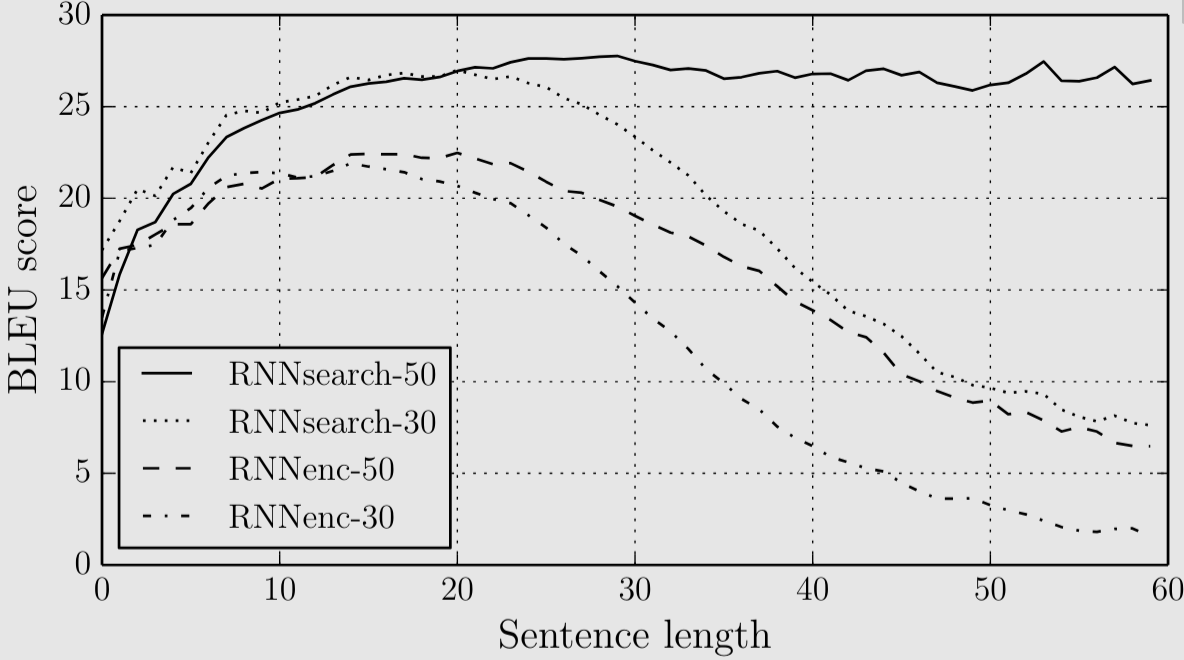
\includegraphics[width=0.66\linewidth]{part1/visuals/enc_dec.png}
    \caption{生成译文的双语评估替补（bilingual evaluation understudy，BLEU）分数随句子长度的变化 \citep{DBLP:journals/corr/BahdanauCB14}。}
    \label{fig:enc-dec-bleu}
\end{figure}

注意力背后的直觉，是在上下文向量中纳入所有编码器隐藏状态的线性组合，而不是只依靠最后一个隐藏状态。这使模型能够回看输入序列中与当前生成词相关的特定部分。通过调整输入词元 $x_i$ 在线性组合中的权重 $a_i$，就能够控制对它分配多少关注，如式~\ref{eq:enc-dec-attention}~所示。这里，$\mathbf{c}_j$ 是第 $j$ 个输出的上下文向量，$h_i$ 表示第 $i$ 个输入词元的隐藏状态。

\begin{equation}
\label{eq:enc-dec-attention}
    \mathbf{c}_{j} = a_1\mathbf{h}_1, \dots, a_n\mathbf{h}_n
\end{equation}

权重 $a$ 通常称为注意力权重，它们并不固定，而是动态计算出来的。一个关键认识是，可以利用隐藏状态 $h_i$，因为它们表示词元或词语的语义。通过比较两个隐藏状态，例如计算余弦相似度，就能够判断它们之间有多相关。{\em 经 softmax 归一化的点积}是一种常用方法：
\begin{enumerate}
    \item 使用点积等相似度函数，将当前解码器状态与每个编码器隐藏状态比较，判断二者匹配程度。
    \item 将这些分数送入 softmax 函数，使其总和为 1，从而在输入词元上形成一个概率分布。
\end{enumerate}
注意力提高了准确性，但循环神经网络的高效计算问题仍未解决。循环神经网络按顺序逐个处理词元，无法充分利用 GPU 中的现代并行计算硬件。为了扩展到大型数据集，需要彻底去掉循环结构：将序列结构改为具有固定上下文宽度的并行结构，同时处理所有词元。这通过\textit{自注意力（self-attention）}实现。数学上，上下文相关嵌入的计算就变为式~\ref{eq:contextualized-embeddings}。
\begin{equation}
\label{eq:contextualized-embeddings}
    \mathbf{a}_3 = \sum_{j=1}^{5} \alpha_{3j} \mathbf{x}_j = \sum_{j=1}^{5} \textsf{softmax}{(\underbrace{\mathbf{x}_3}_{\text{query}} \cdot \underbrace{\mathbf{x}_j}_{\text{key}}}) \underbrace{\mathbf{x}_j}_{\text{value}}
\end{equation}

\begin{equation}
\label{eq:attention}
    \text{Attention}(Q, K, V) = \text{softmax}\left(\frac{QK^T}{\sqrt{d_k}}\right)V
\end{equation}

其中，$Q$ 是表示当前关注内容的矩阵，$K$ 表示提供序列中待比较信息的键，$V$ 是包含实际待提取内容的矩阵，$d_k$ 表示键的维数，用于缩放以防止梯度消失。随着维数 $d_k$ 增大，点积 $QK^T$ 可能变得很大，把 softmax 函数推入梯度很小的区域。除以 $\sqrt{d_k}$ 能抵消这一影响，使训练更加稳定。

注意力矩阵 $Q,K,V$ 合在一起，称为一个注意力{\em 层}或注意力{\em 头}。在实践中，一个注意力层会捕捉词元之间某种特定类型的交互。不过，如果只有一种交互，模型每次就只能关注一种关系，也就是一个注意力{\em 头}所表示的关系。一个词可以涉及许多不同的语言关系，例如句法关系（{\em 这个名词对应哪个动词？}）、语义关系（{\em 这个词是不是某个隐喻的一部分？}）或指称关系（{\em “他”指的是谁？}）。同时使用多个头，就能让模型表示多种关系。某个头可能学会寻找语法结构，另一个头寻找代词，还有一个头寻找实体。各个头并行工作，结果拼接为一个丰富的统一表示。这些头共同组成一层，如式~\ref{eq:multi-head-attention}~所示。

\begin{align}
    \label{eq:multi-head-attention}
    \text{MultiHead}(Q, K, V) &= \text{Concat}(\text{head}_1, \dots, \text{head}_h)W^O \\
    \nonumber \text{where } \text{head}_i &= \text{Attention}(QW_i^Q, KW_i^K, VW_i^V)
\end{align}

\subsection{Transformer}
如何利用注意力机制，构建用于语言建模的架构？下面介绍其中一种：\citet{vaswani2017attention} 在奠基性工作中提出的 Transformer 架构。

注意力机制是 Transformer 架构的核心。图~\ref{fig:transformer}~所示的原始 Transformer 架构，同时包含编码器与解码器。图左侧是编码器堆叠，右侧是解码器堆叠。大多数大语言模型采用仅解码器的 Transformer。

图中每个 {\em Transformer 块（transformer block）}都包含自注意力模块、前馈网络、归一化层，以及从输入通向输出的残差连接。大多数大语言模型会把许多 Transformer 块逐层堆叠起来。例如，根据模型版本不同，GPT-2 包含 12 层或更多层。

\begin{figure}[tb]
    \centering
    % 严格对应原包 transformer_full_architecture.png 的预归一化版本。
% 保留编码器两子层、解码器三子层、全部残差，以及交叉注意力的 V/K/Q 来源。
\begin{tikzpicture}[
    font=\small,
    box/.style={draw,line width=.8pt,rounded corners=3pt,minimum width=2.55cm,minimum height=.55cm,align=center,fill=white},
    norm/.style={box,fill=green!15,draw=green!45!black},
    attn/.style={box,fill=blue!15,draw=blue!55!black,minimum height=.8cm},
    ff/.style={box,fill=yellow!20,draw=yellow!55!black,minimum height=.8cm},
    add/.style={circle,draw,line width=.8pt,fill=white,minimum size=.4cm,inner sep=0pt},
    flow/.style={-{Stealth[length=1.8mm]},line width=.7pt},
    residual/.style={flow,rounded corners=3pt},
    grouping/.style={draw,dashed,line width=.7pt,rounded corners=7pt},
    qkv/.style={font=\scriptsize,fill=white,inner sep=.5pt}
]
% 编码器。
\node[align=center] (source) at (2.8,0) {源序列};
\node[box] (ee) at (2.8,.85) {嵌入／投影};
\node[add] (ep) at (2.8,1.9) {$+$};
\node[align=center] (epos) at (.55,1.9) {位置编码};
\node[norm] (en1) at (2.8,2.95) {归一化};
\node[attn] (ea) at (2.8,4.2) {多头自注意力};
\node[add] (es1) at (2.8,5.2) {$+$};
\node[norm] (en2) at (2.8,6.15) {归一化};
\node[ff] (ef) at (2.8,7.2) {前馈网络};
\node[add] (es2) at (2.8,8.2) {$+$};
\node[norm] (enout) at (2.8,9.2) {归一化};
\draw[flow] (source) -- (ee);
\draw[flow] (ee) -- (ep);
\draw[flow] (epos) -- (ep);
\draw[flow] (ep) -- (en1);
\draw[line width=.7pt] (en1.north) -- (2.8,3.4);
\foreach \xx/\offset/\lab in {2.15/-.65/V,2.8/0/K,3.45/.65/Q}{
  \draw[flow,rounded corners=2pt] (2.8,3.4) -| ([xshift=\offset cm]ea.south);
  \node[qkv] at (\xx,3.6) {\lab};
}
\draw[flow] (ea) -- (es1);
\draw[flow] (es1) -- (en2);
\draw[flow] (en2) -- (ef);
\draw[flow] (ef) -- (es2);
\draw[flow] (es2) -- (enout);
\draw[residual] (2.8,2.4) -- (4.35,2.4) -- (4.35,5.2) -- (es1.east);
\draw[residual] (2.8,5.65) -- (4.35,5.65) -- (4.35,8.2) -- (es2.east);
\draw[grouping] (1.25,2.35) rectangle (4.5,5.65);
\draw[grouping] (1.25,5.65) rectangle (4.5,8.65);
\draw[draw=yellow!60!black,line width=.9pt,rounded corners=10pt] (1.12,2.22) rectangle (4.63,8.78);
\node[align=center] at (.45,5.55) {$N$ 层};

% 解码器。
\node[align=center] (target) at (7.8,0) {移位后的\\目标序列};
\node[box] (de) at (7.8,.85) {嵌入／投影};
\node[add] (dp) at (7.8,1.9) {$+$};
\node[align=center] (dpos) at (10.2,1.9) {位置编码};
\node[norm] (dn1) at (7.8,2.95) {归一化};
\node[attn,fill=red!15,draw=red!55!black] (da) at (7.8,4.2) {掩码多头\\自注意力};
\node[add] (ds1) at (7.8,5.2) {$+$};
\node[norm] (dn2) at (7.8,6.15) {归一化};
\node[attn] (dc) at (7.8,7.5) {多头交叉注意力};
\node[add] (ds2) at (7.8,8.55) {$+$};
\node[norm] (dn3) at (7.8,9.5) {归一化};
\node[ff] (df) at (7.8,10.55) {前馈网络};
\node[add] (ds3) at (7.8,11.6) {$+$};
\node[norm] (dnout) at (7.8,12.65) {归一化};
\node[box] (linear) at (7.8,13.65) {线性层};
\node (pred) at (7.8,14.55) {预测};
\draw[flow] (target) -- (de);
\draw[flow] (de) -- (dp);
\draw[flow] (dpos) -- (dp);
\draw[flow] (dp) -- (dn1);
\draw[line width=.7pt] (dn1.north) -- (7.8,3.35);
\foreach \xx/\offset/\lab in {7.15/-.65/V,7.8/0/K,8.45/.65/Q}{
  \draw[flow,rounded corners=2pt] (7.8,3.35) -| ([xshift=\offset cm]da.south);
  \node[qkv] at (\xx,3.45) {\lab};
}
\draw[flow] (da) -- (ds1);
\draw[flow] (ds1) -- (dn2);
\draw[flow,rounded corners=3pt] (dn2.north) -- (7.8,6.6) -- (8.45,6.6) -- node[qkv,pos=.7] {$Q$} (8.45,7.1);
\draw[line width=.7pt,rounded corners=4pt] (enout.north) -- (2.8,9.85) -- (5.2,9.85) -- (5.2,6.8) -- (7.8,6.8);
\draw[flow] (7.15,6.8) -- node[qkv,pos=.55] {$V$} (7.15,7.1);
\draw[flow] (7.8,6.8) -- node[qkv,pos=.55] {$K$} (7.8,7.1);
\draw[flow] (dc) -- (ds2);
\draw[flow] (ds2) -- (dn3);
\draw[flow] (dn3) -- (df);
\draw[flow] (df) -- (ds3);
\draw[flow] (ds3) -- (dnout);
\draw[flow] (dnout) -- (linear);
\draw[flow] (linear) -- (pred);
\draw[residual] (7.8,2.4) -- (9.35,2.4) -- (9.35,5.2) -- (ds1.east);
\draw[residual] (7.8,5.65) -- (9.35,5.65) -- (9.35,8.55) -- (ds2.east);
\draw[residual] (7.8,9.0) -- (9.35,9.0) -- (9.35,11.6) -- (ds3.east);
\draw[grouping] (6.25,2.35) rectangle (9.5,5.65);
\draw[grouping] (6.25,5.65) rectangle (9.5,9.0);
\draw[grouping] (6.25,9.0) rectangle (9.5,12.05);
\draw[draw=green!45!black,line width=.9pt,rounded corners=10pt] (6.12,2.22) rectangle (9.63,12.18);
\node[align=center] at (10.3,6.9) {$N$ 层};
\end{tikzpicture}

    \caption{Transformer 架构示意图 \citep{godoy_dl_visuals,vaswani2017attention}。}
    \label{fig:transformer}
\end{figure}

现在更仔细地考察 Transformer 架构，请结合图示阅读。完整架构由三大类要素组成：嵌入、Transformer 块与输出概率：
\begin{enumerate}
    \item 嵌入：首先，对输入文本进行词元化，将其投影为低维嵌入向量。再向嵌入中加入位置编码（positional encoding），以保留词序。
    \item Transformer 块：这是架构的主体。大多数模型由多层 Transformer 块组成。在每层中，每个块包含三个要素：
    \begin{itemize}
        \item 自注意力机制：注意力机制允许词元之间建立长距离连接，捕捉上下文信息与词元间关系。多个注意力头使模型能够从不同角度考察这些关系，例如短距离句法联系与更广泛的语义上下文。

        在编码器堆叠中，Transformer 使用自注意力；在解码器堆叠中，则使用掩码自注意力，以避免看到未来的信息。
        \item 多层感知机（multilayer perceptron，MLP）：全连接前馈网络分别独立处理各个词元。注意力层在词元之间建立连接，而多层感知机可以细化每个词元的表示。
        \item 归一化：大多数 Transformer 块还加入了归一化、正则化（dropout）与残差连接等典型深度学习方法，以防止梯度消失或爆炸，提高训练的稳定性。
    \end{itemize}
    \item 输出概率：线性层与 softmax 层将处理后的嵌入转化为概率，用以预测下一个词元。
\end{enumerate}
与 RNN、LSTM 网络等早期方法相比，Transformer 架构具有两项主要优势。基于注意力的 Transformer 支持 (1) 大规模并行处理，以及 (2) 细致的长距离语义连接，也就是同时兼顾速度{\em 与}语义准确性。

自问世以来，Transformer 一直主导着语言建模。在大规模高质量训练语料建成后，基于 Transformer 的大语言模型在问答、数据到文本生成及应用驱动的任务上，取得了令人印象深刻的表现。研究者不断追求更大的模型，期待获得更强能力 \citep{brown2020language}。第~\ref{chap:scaling}~章将讨论如何进一步扩展性能。

Transformer 是一种复杂架构。网上有一些优秀的交互式教程，提供了更多细节；\footnote{例如，参见 \url{https://poloclub.github.io/transformer-explainer/}。}也可以参阅第~\ref{ch:nanochat}~章的案例研究。

\subsection{仅编码器模型（BERT）}
原始 Transformer 模型采用编码器与解码器相结合的结构，而现代模型通常只采用编码器或解码器，因为经验表明，它们各自具有特定优势。

先仔细看看编码器。编码器使用掩码语言建模（masked language modeling，MLM）等技术进行训练，把输入数据压缩为有意义的表示，即嵌入。它们擅长文本分类、情感分析等自然语言理解任务，而解码器则擅长文本生成、改写与摘要等自然语言生成任务。

仅编码器模型的设计目标，是为输入文本产生高质量向量表示，也就是嵌入。解码器具有{\em 因果性}，只能看到先前的词；与之不同，编码器天然是双向的。在编码器中，序列中的每个词元都可以同时关注其他所有词元。这种全局上下文，使模型能够构建输入的复杂语义表示。
训练这类模型时，我们采用掩码语言建模：将大约 15\% 的输入词元替换为特殊词元 \texttt{[MASK]}，让模型学习词表中的哪个词元应当填在这个位置。通常使用一般的交叉熵损失更新模型。掩码语言模型编码器训练的目标，是让模型利用左右两侧的周围上下文，预测被遮住的词。最终，这迫使模型学会语法、语义，甚至一些关于世界的逻辑。

为了改善学习，除了 \texttt{[MASK]} 以外，编码器训练通常还使用若干特殊词元：
\begin{itemize}
    \item \texttt{[CLS]}（classification，分类）：插入序列最开头。经过全部层之后，这个词元的最终状态用作整个序列的汇总表示。
    \item \texttt{[SEP]}（separator，分隔）：告诉模型一个句子在哪里结束、另一个句子在哪里开始，这对问答等任务至关重要。
    \item \texttt{[PAD]}（padding，填充）：确保一个训练批次中的全部序列长度相同。
\end{itemize}
最著名的仅编码器模型，或许就是{\em 基于 Transformer 的双向编码器表示（bidirectional encoder representations from transformers）}，更广为人知的名称是 BERT~\citep{devlin2018bert}。BERT 及其后继模型 RoBERTa \citep{liu2019roberta}、ALBERT~\citep{lan2019albert} 等仅编码器模型，已经得到广泛使用。

仅编码器模型非常适合迁移学习（transfer learning）：先对输入进行嵌入，再针对下游任务微调，例如某个应用领域的分类任务。构建仅编码器模型的流程包括两个阶段：
\begin{enumerate}
    \item 预训练：首先在包含数十亿词的大型语料上训练模型。例如，模型可能学到 \textit{King} 与 \textit{Man} 有关，\textit{Queen} 与 \textit{Woman} 有关。此时模型还不知道如何完成具体工作，只是在学习英语。预训练成本很高，可能需要很长时间，例如数周或数月。
    \item 微调：接着，取出预训练模型，在其顶部增加一个较小的分类层，通常称为\textit{分类头（classification head）}。随后，在特定任务数据上再次训练整个模型，例如垃圾信息检测或情感分析。由于模型已经理解语言，通常只需要几千个样例，就能成为新任务的专家。微调成本较低，可能只需数小时或数分钟；而从零开始训练特定任务，则需要大型数据集与大量训练时间。
\end{enumerate}
介绍了仅编码器模型后，下面转向仅解码器模型。

\subsection{仅解码器模型（GPT）}
语言生成任务使用仅解码器模型。解码器通过自回归训练来重建数据或生成序列，通常一次生成一个词元。后续词元依赖迄今已经生成的内容，这种自回归依赖是一种\textit{因果注意力（causal attention）}。我们不能借助未来词元来作出最佳预测。
在编码器中，一个词可以看到右边的词；在解码器中，这严格禁止。我们使用前瞻掩码（look-ahead mask），通常是一个三角矩阵，将未来词元的注意力分数设为 $-\infty$。如果模型要在短语 \textit{The boy ate the...} 中预测 \textit{apple}，就不应让它看到训练数据中的 \textit{apple}。解码器必须完全依靠前面的上下文。因此，编码器采用掩码语言建模，解码器则采用通常的\textit{因果语言建模（causal language modeling）}，如下一章的式~\ref{eq:lm}~所示。

由此，从编码器转向解码器时，预训练与微调的关系会略有变化：解码器在预训练中学习预测下一个词，随后用相同的损失函数、另一类数据进行微调。这使我们能够采用{\em 上下文学习（in-context learning，ICL）}，也称提示学习：由于解码器经过训练能够续写序列，你只需提供提示，也就是上下文，它便能生成回答，无须更新权重。可以说，它们是在从提示中的例子学习 \citep{brown2020language}。大型解码器能够通过上下文学习便捷地使用，无须进行昂贵的特定任务训练或微调，这使人们对上下文学习产生了浓厚兴趣。

仅解码器模型，例如{\em 广义预训练 Transformer（generalized pretrained transformer，GPT）}系列 \citep{radford2018improving,radford2019language,brown2020language,ouyang2022training,achiam2023gpt}，已经取得很大成功，如今在社会中广泛使用。此外，还出现了许多其他模型，既有开放模型，也有封闭模型。上述训练机制共同构成现代大语言模型训练流程的基础，第~\ref{chap:pipeline}~章将进一步详述。

\section{结语}
本章回顾了自然语言处理从语言学基础到支撑当今大语言模型的神经网络架构这一非凡演进。我们指出，人类语言本身就很复杂，既有精细的句法与形态规则，也有深层的语义和语用细微差别。现代自然语言处理的突破，经历了符号、统计、神经网络这一系列范式转变，为当代语言模型提供了基本构件：稠密嵌入、注意力机制，以及数据量、模型规模与计算能力的增长。编码器模型适合自然语言理解，解码器模型适合自然语言生成。两者都通过预训练与微调来训练，而解码器还支持基于提示的上下文学习。

\subsection{尚待解决的挑战}
虽然现代大语言模型的表现令人印象深刻，也有许多有用的应用场景，但仍存在重要挑战。理解这些挑战，对于识别研究空白、构建更稳健的系统至关重要；这些问题同样与智能体大语言模型有关。

\paragraph{性能扩展}
当前语言建模采用{\em 扩展定律（scaling law）}这一假设：通过更多参数、更多数据与更多计算这三者，取得更好的泛化能力。不过，进一步扩展也带来显著挑战。要达到最先进的性能，可能需要具有数十亿参数的模型，训练所需的计算费用达数百万美元，并产生很大的环境影响。如何用高效架构取得更好的泛化，也就是完成未专门训练过的任务的能力，仍是一个开放问题。当前研究正在探索模型剪枝与量化，两者都会在第~\ref{chap:scaling}~章介绍。此外，合成数据生成（见第~\ref{chap:synthetic-data}~章）旨在不增加训练数据的情况下，提高泛化能力；但模型大小与泛化能力之间的最佳平衡点，仍然难以确定。

\paragraph{数据稀缺}
大多数自然语言处理训练数据集都是为英语构建的，主要基准测试也如此，例如用于通用语言理解的 GLUE \citep{wang2018glue}，以及用于问答的 SQuAD \citep{rajpurkar2016squad}。数据通常通过大规模网页抓取积累。汉语、印地语等其他高资源语言，也能够受益于这种方法；荷兰语或弗拉芒语等低资源语言，则缺乏从零训练现代 Transformer 所需的数字足迹与文化内容积累。模型会继承训练数据中的文化细微差别，因此，非英语使用者往往会遇到性能下降，或偏向西方视角与语言规范的算法偏见。

\paragraph{多语言能力}
由于可用资源不同，自然语言处理很少能为每种语言提供通用方案。例如，把模型在英语上的成功推广到其他语言，就会引入多方面的语言学复杂性。土耳其语、芬兰语、阿拉伯语等其他语言，在形态上可能更丰富，能够通过动词或名词的前后缀传达大量信息。土耳其语中的一个词，可能对应英语中的一整句话。没有在这些语言上训练过的模型，无法反映这种语言丰富性。

此外，不同语言可能使用不同字符集与文字体系，处理非拉丁文字时便会遇到问题，例如汉语的语素文字，或希伯来语与阿拉伯语的辅音文字。这些语言需要新的词元化与嵌入策略，以形成有意义的子词。

\paragraph{语言演变}
语言是活的，其演变速度快于模型重新训练的速度。这带来的问题之一，就是词表外问题。即使使用字节对编码 \citep{gage1994new} 或 WordPiece \citep{song2021fast} 等子词词元化方法，模型仍难以处理训练截止时尚不存在的新词、俚语、技术行话或名称。此外，一个在 2022 年训练的模型，可能无法理解 2026 年全球事件或文化变化的背景，例如，什么是“Z 世代凝视”（Gen Z stare）？如何构建能够更新知识、又不遗忘旧信息的持续学习系统，避免灾难性遗忘（catastrophic forgetting），仍是一项开放挑战 \citep{wu2024continual}。

\paragraph{超越文本的词元化}
为了理解传统语境之外的信息，人们正在努力打通文本与其他模态之间的边界。提供这种上下文的一项挑战，是多模态表示：将图像、音频、视频与文本表示在同一个潜在空间中。文本是离散的，由词语或字符组成；音频与视频则是连续信号，必须采样并量化。要把一帧视频或一段波形映射为词元，使语言模型能够将其与文本一同处理，需要视觉 Transformer（Vision Transformer，ViT）\citep{han2022survey} 或对比式语言—图像预训练（Contrastive Language-Image Pre-training，CLIP）\citep{radford2021learning} 等复杂架构。第~\ref{chap:world}~章将讨论多模态模型。

\paragraph{可解释性}
最后，一个重要的开放问题是，这些模型内部究竟如何工作。虽然我们能够测量模型是否有效，却往往难以解释它为何给出某个特定回答。此外，模型经常出错，或产生幻觉，以令人信服的方式给出错误答案。对于军事、法律或医疗自然语言处理等高风险应用，缺乏透明性应当成为采用语言模型的一项重要障碍。第~\ref{chap:mi}~章将讨论可解释语言模型的相关技术，例如机制可解释性。

除了这些挑战，语言建模还面临伦理对齐、长篇逻辑推理等许多其他社会技术挑战。随着自然语言处理不断发展，这些开放问题构成了一片持续变化的前沿：解决一个挑战，往往又会为下一代学生、研究者与工程师揭示一系列更深的问题。

\subsection{展望}
本章讨论了语言建模的基础，从早期起步一直讲到现代解码器模型。现在，我们已经准备好进一步深入智能体大语言模型。下一章将更详细地介绍大语言模型训练流程如何运作。

\bibliographystyle{plainnat}
\bibliography{agenticbook,refs,case,synthetic}
